\documentclass{article}
\usepackage{amsmath}
\usepackage{amssymb}
\usepackage[dvipsnames]{xcolor}
\usepackage{graphicx}
\usepackage{tikz}
\usepackage{pgfplots}
\usetikzlibrary{arrows}
\usetikzlibrary{datavisualization.formats.functions}
\usepgfplotslibrary{fillbetween}
\usetikzlibrary{patterns}
\usepackage[margin=1.2in]{geometry}
\usepackage[skins,theorems]{tcolorbox}
\tcbset{highlight math style={enhanced,
  colframe=blue,colback=white,arc=0pt,boxrule=1pt}}

\newcommand*\eval[3]{\left[#1\right]_{#2}^{#3}}
\newcommand*\pbar[0]{\,|\,}
\newcommand*\var[0]{\text{Var}}

\begin{document}

\title{Theory of Probability HW \#7}
\author{Ozaner Hansha}
\date{November 11, 2019}
\maketitle

\subsection*{Problem 1}
\noindent\textbf{Problem:} Is the following function a joint pdf?
\begin{equation*}
    f(x,y)=\begin{cases}
        \frac{1}{2},&0<y<x<1\\
        0,&\text{otherwise}
    \end{cases}
\end{equation*}

% If so, let it be the joint pdf of both $X$ and $Y$, and compute the marginal densities of $X$ and $Y$.
% \bigskip

\noindent\textbf{Solution:} If $f(x,y)$ is a joint pdf, then the following definite integral must evaluate to 1:
\begin{align*}
    \int_{-\infty}^\infty\int_{-\infty}^\infty f(x,y)\mathop{dy}\mathop{dx}&=\int_0^1\int_0^x \frac{1}{2}\mathop{dy}\mathop{dx}\\
    &=\int_0^1\eval{\frac{y}{2}}{0}{x}\mathop{dx}\\
    &=\int_0^1\frac{x}{2}\mathop{dx}\\
    &=\eval{\frac{x^2}{4}}{0}{1}=\frac{1}{4}\not=1
\end{align*}

\tcbhighmath[boxrule=0.4pt,colframe=blue,colback=blue!10!white]{\text{And so $f(x,y)$ is \textit{not} a joint pdf.}}

\subsection*{Problem 2}
\noindent\textbf{Problem:}  Sonia and Natasha are supposed to meet at a certain location around 5:30 pm. Sonia arrives at some time uniformly distributed between 5:00 pm and 6:00 pm, while Natasha arrives at some time uniformly distributed between 5:15 pm and 6:00 pm. Given that Natasha arrives first, what is the probability that she will not have to wait for more than 10 minutes for Sonia?
\bigskip

\noindent\textbf{Solution:} Let $S$ be the time in minutes after 5:00 pm that Sonia arrives, and $N$ be the time that Natasha arrives. We then have the following \textit{independent}, as neither one's arrival time affects the other, random variables:
\begin{equation*}
    S\sim\mathcal U(0,60)\,\,\,\,\,\,\,\,\,\,\,\,\,\,\,\,N\sim\mathcal U(15,60)
\end{equation*}

Our desired probability is thus given by:
\begin{align*}
    P(N-S\le 10\pbar N\le S)&=\frac{P(N-S\le 10, N\le S)}{P(N\le S)}\tag{def. of conditional prob.}\\
    &=\frac{\iint\limits_{s-n\le10\atop n\le s}f(n,s)\mathop{ds}\mathop{dn}}{\iint\limits_{n\le s}f(n,s)\mathop{dn}\mathop{ds}}\tag{joint pdf}\\
    &=\frac{\iint\limits_{s-n\le10\atop n\le s}f_N(n)f_S(s)\mathop{ds}\mathop{dn}}{\iint\limits_{n\le s}f_N(n)f_S(s)\mathop{dn}\mathop{ds}}\tag{independence}\\
    &=\frac{\frac{1}{45}\cdot\frac{1}{60}}{\frac{1}{45}\cdot\frac{1}{60}}\frac{\iint\limits_{s-n\le10\atop n\le s}\mathop{ds}\mathop{dn}}{\iint\limits_{n\le s}\mathop{dn}\mathop{ds}}\tag{uniform pdf}\\
    &=\frac{\iint\limits_{s-n\le10\atop n\le s}\mathop{ds}\mathop{dn}}{\iint\limits_{n\le s}\mathop{dn}\mathop{ds}}
    % &=\frac{\iint\limits_{s-n\le10\atop n\le s}\mathop{ds}\mathop{dn}}{\int_{15}^{60}\int_{15}^{s}\mathop{dn}\mathop{ds}}\tag{$15\le n\le s\le 60$}\\
    % &=\frac{\iint\limits_{s-n\le10\atop n\le s}\mathop{ds}\mathop{dn}}{\int_{15}^{60}x-15\mathop{ds}}=\frac{\iint\limits_{s-n\le10\atop n\le s}\mathop{ds}\mathop{dn}}{\eval{\frac{x^2}{2}-15x}{15}{60}}\\
    % &=\frac{2}{2025}\iint\limits_{s-n\le10\atop n\le s}\mathop{ds}\mathop{dn}
\end{align*}

Now all that remains is to find the areas of integration of both the numerator and denominator. To illustrate them, we present a graph of the relevant conditions in the $sn$ plane:

\begin{center}
    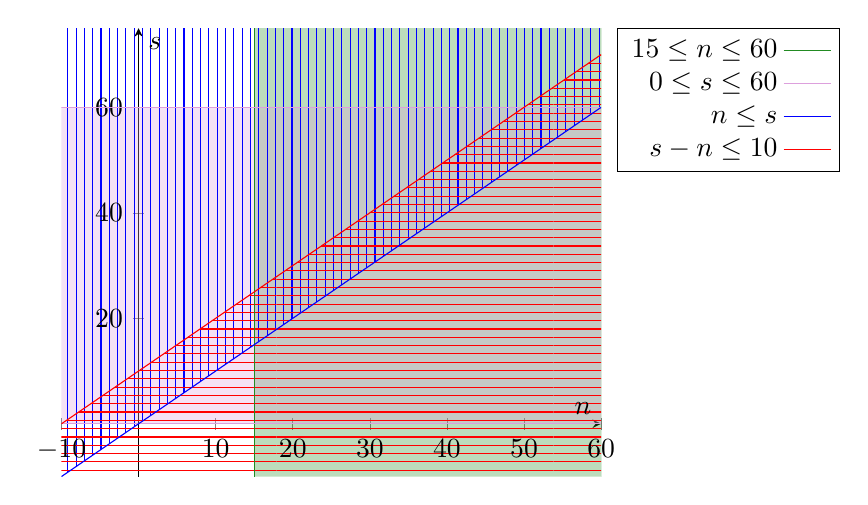
\begin{tikzpicture}
    \begin{axis}[
        xlabel=$n$,
        ylabel=$s$,
        xmin=-10,xmax=60,
        ymin=-10,ymax=75,
        axis lines=center,
        legend pos=outer north east,
        legend style={legend cell align=right,legend plot pos=right}] 

    \addplot[ForestGreen,forget plot] coordinates{(15,-10) (15,75)};
    \addplot[ForestGreen] coordinates{(60,-10) (60,75)};
    \addlegendentry{$15\le n\le60$}
    \plot[name path=P1, thick,samples=100,domain=-10:60,
    forget plot,draw=none] {75};
    \plot[name path=P2,thick,samples=100,domain=-10:60,
        forget plot,draw=none] {-10};
    \addplot[fill=ForestGreen,
        opacity=.3,
        forget plot,
        % pattern=horizontal lines,
        pattern color=ForestGreen]
        fill between [of=P1 and P2, soft clip={domain=15:60}];

    \addplot[color=Plum,domain=-10:60,samples=100,forget plot] {0};
    \addplot[color=Plum,domain=-10:60,samples=100] {60};
    \addlegendentry{$0\le s\le60$}
    \plot[name path=R1, thick,samples=100,domain=-10:60,
    forget plot,draw=none] {60};
    \plot[name path=R2,thick,samples=100,domain=-10:60,
        forget plot,draw=none] {0};
    \addplot[fill=Plum,
        opacity=.3,
        forget plot,
        % pattern=vertical lines,
        pattern color=Plum]
        fill between [of=R1 and R2, soft clip={domain=-10:60}];

    \addplot[color=blue,domain=-10:60,samples=100] {x};
    \addlegendentry{$n\le s$}
    \plot[name path=B1, thick,samples=100,domain=-10:60,
        forget plot,draw=none] {x};
    \plot[name path=B2,thick,samples=100,domain=-10:60,
        forget plot,draw=none] {75};
    \addplot[fill=blue,
        % opacity=.8,s
        forget plot,
        pattern=vertical lines,
        pattern color=blue]
        fill between [of=B1 and B2, soft clip={domain=-10:60}];

    \addplot[color=Red,domain=-10:60,samples=100] {x+10};
    \addlegendentry{$s-n\le10$}
    \plot[name path=G1, thick,samples=100,domain=-10:60,
        forget plot,draw=none] {x+10};
    \plot[name path=G2,thick,samples=100,domain=-10:60,
        forget plot,draw=none] {-10};
    \addplot[fill=Red,
        % opacity=.8,
        forget plot,
        pattern=horizontal lines,
        pattern color=Red]
        fill between [of=G1 and G2, soft clip={domain=-10:60}];

    \end{axis}
    \end{tikzpicture}
\end{center}

The area of the denominator is given by the blue right triangle that satisfies the first three listed conditions:
\begin{equation*}
    \iint\limits_{n\le s}\mathop{dn}\mathop{ds}=\frac{(60-15)^2}{2}=\frac{2025}{2}
\end{equation*}

The area of the numerator is the trapezoidal shape contained in aforementioned right triangle that is further bounded by the last condition. The legs of this isosceles trapezoid, i.e. the green and purple sides, are simply $c=10$. The top base, i.e. the red side, is given by:
\begin{equation*}
    a=\|(50,60)-(15,25)\|=\|(35,35)\|=35\sqrt{2}
\end{equation*}

Similarly the bottom base, i.e. the blue side, is given by:
\begin{equation*}
    b=\|(60,60)-(15,15)\|=\|(45,45)\|=45\sqrt{2}
\end{equation*}

The semiperimeter $s$ of the trapezoid is given by:
\begin{equation*}
    s=\frac{a+b+2c}{2}=\frac{35\sqrt{2}+45\sqrt{2}+20}{2}
\end{equation*}

Plugging these into Brahmagupta's formula for an isosceles trapezoid, we find the area to be:
\begin{equation*}
    \iint\limits_{s-n\le10\atop n\le s}\mathop{ds}\mathop{dn}=\sqrt{(s-a)(s-b)(s-c)^2}=10\sqrt{30\sqrt{7}+79}
\end{equation*}

And so our final answer is given by:
\begin{align*}
    P(N-S\le 10\pbar N\le S)&=\frac{\iint\limits_{s-n\le10\atop n\le s}\mathop{ds}\mathop{dn}}{\iint\limits_{n\le s}\mathop{dn}\mathop{ds}}\\
    &=\frac{2}{2025}\left(10\sqrt{30\sqrt{7}+79}\right)\\
    &=\tcbhighmath[boxrule=0.4pt,colframe=blue,colback=blue!10!white]{\frac{4}{405}\sqrt{30\sqrt{7}+79}\approx0.124292}
\end{align*}

\subsection*{Problem 3}
\noindent\textbf{Problem:} At a fundraiser, the individual dontations of 200 people are independent random variables, each of which is uniformly distributed over \$0 to \$200. Give an expression for the probability that exactly 5 people donate at most \$10 each.
\bigskip

\noindent\textbf{Solution:} Let $X$ be the amount any particular individual donates. It is given by:
\begin{equation*}
    X\sim\mathcal U(0,200)
\end{equation*}

The probability that any particular individual donates at most \$10 is given by:
\begin{equation*}
    P(X\le 10)=F_X(10)=\frac{10}{200}=\frac{1}{20}
\end{equation*}

Given 200 such individuals, each independently donating money with the above distribution, the number of donors $Y$ who donate at most \$10 is given by the following binomial distribution:
\begin{equation*}
    Y\sim B\left(200,\frac{1}{20}\right)
\end{equation*}

And so our desired probability is given by:
\begin{align*}
    P(Y=5)&=p_Y(5)\tag{def. of pmf}\\
    &=\tcbhighmath[boxrule=0.4pt,colframe=blue,colback=blue!10!white]{\binom{200}5 \left(\frac{1}{20}\right)^5\left(\frac{19}{20}\right)^{195}\approx0.035896}\tag{binomial distribution}
\end{align*}

\textit{If desired, a more numerically stable approximation of the above probability could be found via the normal approximation.}

\subsection*{Problem 4}
\noindent\textbf{Problem:} It is observed that the scores of a typical student in Math 477 on Exam I are normally distributed with mean 50 and standard deviation 5, while their scores on Exam II are independently and normally distributed with mean 55 and standard deviation 12. Suppose you are a typical student. What is the probability that the total of your scores on Exam I and II
exceeds 150?
\bigskip

\noindent\textbf{Solution:} Let the random variables $E_1$ and $E_2$ be the score of a typical student on exam 1 and 2 respectively. They are given by:
\begin{equation*}
    E_1\sim\mathcal N(50,\underbrace{25}_{5^2})\,\,\,\,\,\,\,\,\,\,\,\,\,\,\,\,E_2\sim\mathcal N(55,\underbrace{144}_{12^2})
\end{equation*}

Let the total score $T=E_1+E_2$. Recall that the sum of two normally distributed random variables is itself, normally distributed with $\mu=\mu_1+\mu_2$ and $\sigma^2=\sigma^2_1+\sigma^2_2$. We thus have:
\begin{equation*}
    T\sim\mathcal N(\underbrace{105}_{50+55},\underbrace{169}_{5^2+12^2})
\end{equation*}

And so, our desired probability is given by:
\begin{align*}
    P(T>150)&=1-P(T\le150)\tag{complement}\\
    &=1-F_T(150)\tag{def. of cdf}\\
    &=1-\Phi\left(\frac{150-105}{\sqrt{169}}\right)\tag{unit normal distribution}\\
    &=\tcbhighmath[boxrule=0.4pt,colframe=blue,colback=blue!10!white]{1-\Phi\left(\frac{45}{13}\right)\approx0.000269}
\end{align*}

\subsection*{Problem 5}
\noindent\textbf{Problem:} A point $(X, Y)$ in the Cartesian plane is uniformly distributed within the unit circle when $X$ and $Y$ have the following joint density:
\begin{equation*}
    f(x,y)=\begin{cases}
        \frac{1}{\pi},&x^2+y^2\le1\\
        0,&\text{otherwise}
    \end{cases}
\end{equation*}

Find the marginal densities $f_X$ and $f_Y$ and state whether $X$ and $Y$ are independent or not.
\bigskip

\noindent\textbf{Solution:} The marginal pdf of $X$, when $x^2\le 1$, is given by:
\begin{align*}
    f_X(x)&=\mkern-10mu\int\limits_{x^2+y^2\le 1}\mkern-19muf(x,y)\mathop{dy}\tag{def. of marginal pdf}\\
    &=\frac{1}{\pi}\mkern-15mu\int\limits_{x^2+y^2\le 1}\mkern-15mu\mathop{dy}\tag{uniform distribution}\\
    &=\frac{1}{\pi}\int_{-\sqrt{1-x^2}}^{\sqrt{1-x^2}}\mathop{dy}\\
    &=\frac{2\sqrt{1-x^2}}{\pi}
\end{align*}

By symmetry, we know that the marginal distribution of $Y$ is the same. And so, the complete marginal pdfs of both $X$ and $Y$ are given by:
\begin{equation*}
    \tcbhighmath[boxrule=0.4pt,colframe=blue,colback=blue!10!white]{f_X(a)=f_Y(a)=\begin{cases}
        \frac{2\sqrt{1-a^2}}{\pi}, &a^2\le 1\\
        0,&\text{otherwise}
    \end{cases}}
\end{equation*}

Now we show that the two random variables are \textit{not} independent. Recall that two random variables $X$ and $Y$ are only independent if the product of their pdfs is equal to their joint pdf for all inputs:
\begin{equation*}
    f(x,y)=f_X(x)f_Y(y)\,\,\,\,\,\,\,\,\,\,\,\,\,\,\,(x,y)\in\mathbb R^2\\
\end{equation*}

However, we can prove that this is not the case for our unit circle distribution via a simple counterexample. Consider the point $(0.5,0.5)$:
\begin{align*}
    f_X(0.5)f_Y(0.5)&=\left(\frac{2\sqrt{1-(0.5)^2}}{\pi}\right)\\
    &=\left(\frac{2\sqrt{0.75}}{\pi}\right)\not=\frac{1}{\pi}=f(0.5,0.5)
\end{align*}

\tcbhighmath[boxrule=0.4pt,colframe=blue,colback=blue!10!white]{\text{And so, $X$ and $Y$ are \textit{not} independent.}}

\subsection*{Problem 6}
\noindent\textbf{Problem:} There were 8 questions on Exam I. Out of these, each student was allowed to choose 2 questions for resubmission. Suppose students made their choices independently and randomly (i.e., each student chose 2 out of the 8 questions completely at random). What is the expected number of problems not chosen by any of the 70 students in the classroom?
\bigskip

\noindent\textbf{Solution:} Let the random variable $X_{ij}$, with $i<j$, denote the number of times both questions $i$ and $j$ were chosen by a student. Since each student chooses independently we have:
\begin{equation*}
    X_{ij}\sim B\left(70,\frac{1}{\binom{8}{2}}\right)
\end{equation*}

Now let the random variable $X_i$ denote the number of times the question $i$ was chosen by a student. It is defined as:
\begin{equation*}
    X_i=\sum_{j\in[1..8]\atop{i<j}}X_{ij}
\end{equation*}

Now note that $X_{ij}>0$ since a pair of questions can't be chosen less than 0 times. As a result, the only way for $X_i=0$ is if each $X_{ij}=0$ for all $i<j$. And since each $X_{ij}$ is i.i.d., we have the following probability:

\begin{align*}
    P(X_i=0)&=\prod_{j\in[1..8]\atop{i<j}}P(X_{ij}=0)\tag{independent}\\
    &=P(X_{ij}=0)^{8-i}\tag{identical}\\
    &=\left(\binom{70}{0}\left(\frac{1}{\binom{8}{2}}\right)^0\left(1-\frac{1}{\binom{8}{2}}\right)^{70}\right)^{8-i}\tag{binomial distribution}\\
    &=\left(1-\frac{1}{\binom{8}{2}}\right)^{560-70i}
\end{align*}

Now, letting $Y$ be the number of questions that haven't been chosen by anyone, we have the following expectation:
\begin{align*}
    Y&=\sum_{i=1}^8 \mathbf{1}_{X_i=0}\\
    E[Y]&=\sum_{i=1}^8 E[\mathbf{1}_{X_i=0}]\tag{linearity of expectation}\\
    &=\sum_{i=1}^8 P(X_i=0)\tag{expectation of indicator}\\
    &=\tcbhighmath[boxrule=0.4pt,colframe=blue,colback=blue!10!white]{\sum_{i=1}^8 \left(1-\frac{1}{\binom{8}{2}}\right)^{560-70i}\approx1.08509}
\end{align*}

\end{document}